\begin{longtabu}to\textwidth{@{}l|cp{280pt}p{200pt}X}
	{\bfseries Verteilungsfunktion:}\\
	%.%%%%%%%%%%%%%%%%%%%%%%
	%.%%.Dichtefunktion %{{{
	%.%%%%%%%%%%%%%%%%%%%%%%
	Dichtefunktion für $X\sim N(0,1)$: $\phi(\frac{x-\mu}{\sigma})$
	&$\stackrel{\text{1. Abltg.}}{=}$&
	$
	\underbrace{\frac{\partial}{\partial x}\left( \frac{x-\mu}{\sigma}
	\right)}_{\text{innere Ableitung}} \cdot \underbrace{\Phi'\left( \frac{x-\mu}{\sigma}
	\right)}_{\text{äußere Ableitung}}
	$&
	Die erste Ableitung der Verteilungsfunktion F(x) wird als
	 Dichtefunktion von x bezeichnet: $\frac{1}{\sigma\sqrt{2\pi}}\cdot e^{-\frac{x^2}{2\sigma^2}}$\vspace{3ex}
	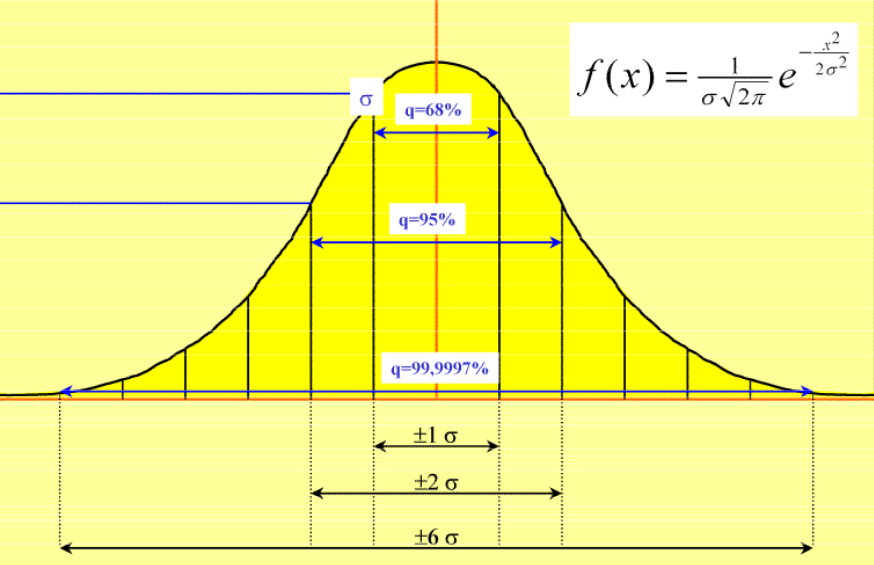
\includegraphics[width=28ex]{./sources/normvert_funkt_dichte}\\\\
 % \includegraphics*[width=15em,height=22ex]{./sources/normvert_funkt_dichte}\\
	%}}}

	{\bfseries Zu zeigen ist:}\\
	%.%%.a^2(Var(X)) %{{{
	%.%%%%%%%%%%%%%%%%%%%
	$Var(aX+b)=a^2Var(X)$&&$E\left(aX+\textcolor{red}{b} - \underbrace{E(aX+\textcolor{red}{b})}_{=aEX}\right)^2$&Die Konstante 'b' lässt sich herauskürzen\\%{{{%}}}%{{}}
	%.%%.Var(X)+Var(Y)+2cov(X,Y) %{{{
	%.%%%%%%%%%%%%%%%%%%%%%%%%%%%%%%%
	\\\\$Var(X+Y)=Var(X)+Var(Y)+2cov(X,Y)$&&$E\left(X+Y-E(X+Y)\right)^2$&$E(X+Y)=EX+EY$, aber\\
	&&&$Var(X+Y)\neq Var(X)+Var(Y)$\\
	&=&$E\underbrace{\left(X+Y -
	EX-EY\right)^2}_{\lbrack(X-EX)+(Y-EY)\rbrack^2}$\\
	&$\stackrel{\text{\tiny
	bin.~Form.}}{=}$&$(X-EX)^2+(Y-EY)^2+2\textcolor{blue}{E\mathbf\lbrack}(X-EX)(Y-EY)\textcolor{blue}{\mathbf\rbrack}$\\
	&=&$Var(X)+Var(Y)+2\cdot cov(X,Y)$
	%}}}
	%.%%.ac*cov(X,Y) %{{{
	%.%%%%%%%%%%%%%%%%%%%
	\\\\$cov(aX+b,cY+d)=ac\cdot cov(x,y)$&$\stackrel{\text{\tiny
	def}}{=}$&$E\lbrack\left(aX+\textcolor{red}{b}-E(aX+\textcolor{red}{b})\right)\left(cY+\textcolor{red}{d}-E(cY+\textcolor{red}{d}\right))\rbrack$\\
	&=&$E \lbrack a(X-EX) \cdot c(Y-EY) \rbrack $\\
	&=&$ac\underbrace{E(X-EX)(Y-EY)}_{cov(X,Y)}$
	%}}}
	%.%.Cov(X,Y) = 0 %{{{
	%.%%%%%%%%%%%%%%%%%%%
	\\\\
	$\underbrace{Cov(X,Y)=0}_{\text{wenn }X\bot Y \text{ und gemeinsam
	absolut stetig verteilt!}}$\vspace{10ex}
	&$\Rightarrow$&
	{$\!\begin{aligned} % http://tex.stackexchange.com/q/98482/16595 
				E(X,Y)=&\int^{\infty}_{-\infty}\int^{\infty}_{-\infty}xy\underbrace{f(x,y)}_{f_x(x)f_y(y)}dxdy\\
					&\int^{\infty}_{-\infty}\int^{\infty}_{-\infty}xf_x(x)dx\cdot yf_y(y)dy\\
	&=E(X)\;\cdot\;E(Y)
	\end{aligned}$}&
Da $Cov(X,Y)=\overbrace{E(XY)-EXEY}^{\text{Verschiebungssatz}}$ ist $Cov=0$, falls X u Y unabh (!)\\
	%}}}
\end{longtabu}
